\documentclass[letterpaper]{article}

% default margins are gargantuan
\usepackage[bottom=1cm, right=1cm, left=1cm, top=1cm]{geometry}
\pagenumbering{gobble}

\usepackage{savesym}
\usepackage{multirow}
\usepackage{makecell}
\usepackage{leadsheets}
% leadsheets and gchords both have \chord so we have to save one to prevent collision
\savesymbol{chord}
\usepackage{gchords}
\usepackage{musixtex}
\usepackage{tikz}

\def\musicintext#1{
  {\let\extractline\relax
   \smallmusicsize \nobarnumbers
   \staffbotmarg0pt
   \startextract\addspace{-\afterruleskip}#1\endextract}}

\begin{document}

{
\centering
\begin{tabular}{ p{3cm} p{2cm} p{3cm} p{2cm} c c }
    \multicolumn{6}{c}{Jazz Chords} \\
    \hline
        \multirow{6}{*}{Major Seventh} &
        \multirow{6}{*}{\writechord{Cmaj7}} & &
        \multirowcell{6}{ \raisebox{0ex}[5ex][4ex]
            {\musicintext{\staffbotmarg2\Interligne
            \Notes \zw c\zw e\zw g\zw i\en}} } &
        \multirowcell{6}{ \begin{tikzpicture}
                \node[anchor=south west,inner sep=0] (image) at (0,0) {
                    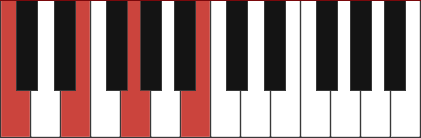
\includegraphics[width=0.2\textwidth]{assets/cmaj7.png}};
            \end{tikzpicture} } &
        \multirowcell{6}{\chord{t}{n,f3p3,f2p2,n,f1p1,n}{C}} \\
        & & • Major Seventh & & & \\
        & & • Perfect Fifth & & & \\
        & & • Major Third & & & \\
        & & • Root & & & \\
        & & & & & \\
    \hline
\end{tabular}\par
}

\end{document}